\subsection{DNA Cloning}
The transformation with the new constructs was validated by sequencing following the mini-preparation. All clones showed 100\% sequence identity with the designs. The concentrations of the plasmids after the midi preparation were measured as \SI{605}{\nano\gram\per\micro\litre} (d29-A), \SI{335}{\nano\gram\per\micro\litre} (S-Tag-A), and \SI{300}{\nano\gram\per\micro\litre} (S-Tag-B), corresponding to yields of \SI{302}{\micro\gram}, \SI{167}{\micro\gram}, and \SI{150}{\micro\gram}.

\subsection{Protein Analysis}
\subsubsection{eYFP Yield by Fluorescence}
For an estimate of the protein yield in the cell-free expression mix, a fluorescence analysis of a cell-free expression setup expressiong Strep-eYFP was conducted. The calibration showed a linear trend with a coefficient of determination of $R^2 = 0.98$ (\autoref{fig:calibration_eyfp}). Applying the linear model to the sample values, the concentration of Strep-eYFP in the reaction mixture was estimated as \SI{295}{\micro\gram\per\milli\litre}.

\subsubsection{Coomassie Staining and Western Blot} 
Coomassie staining and Western Blot were conducted both directly after the cell-free expression and after the following CaptoCore purification. For each setting, two blots were developed, one using an anti-PVX antibody, and one using an anti-S-Tag antibody. 

For the samples from cell-free expression (\autoref{fig:blot_alice}), the Coomassie Staining shows a wide range of bands. For the samples from ALiCE setups expressing d29-A, S-Tag-A, and S-Tag-B, the pattern looks very similar to that of the non-template control. The sample expressing Strep-eYFP has a notable band at a height corresponding to ~\SI{30}{\kilo\Dalton}, similar to the single band in the Strep-eYFP control. The track containing the S-Tag-CP-PVX control also displays a single band at ~\SI{29}{\kilo\Dalton}, slightly lower than that of the Strep-eYFP control. The sample from the ALiCE setup expressing PVX CP presents a band ~\SI{29}{\kilo\Dalton} as well. 

In the Western Blot based on the anti-PVX antibody, the samples from the ALiCE expressions of d29-A, S-Tag-A, and PVX CP show strong bands at ~\SI{25}{\kilo\Dalton}, ~\SI{31}{\kilo\Dalton}, and ~\SI{29}{\kilo\Dalton}. The band for the expressed PVX CP is particularly strong. The sample from S-Tag-B shows a faint band at ~\SI{28}{\kilo\Dalton}. The control S-Tag-CP-PVX has two bands visible in the blot, a stronger band at ~\SI{28}{\kilo\Dalton}, and a less prominent one at ~\SI{30}{\kilo\Dalton}. In all samples, the observed bands migrated to higher molecular weights than the theoretical molecular weights of \SI{22.6}{\kilo\Dalton} (d29-A), \SI{26.9}{\kilo\Dalton} (S-Tag-A), \SI{26.8}{\kilo\Dalton} (S-Tag-B), \SI{25.1}{\kilo\Dalton} (PVX CP), and \SI{26.9}{\kilo\Dalton} (S-Tag-CP-PVX).

In the blot using the anti-S-Tag antibody, the tracks containing samples from the expression of S-Tag-A and S-Tag-B show a strong signal. For S-Tag-A, the blot shows strong lines at ~\SI{31}{\kilo\Dalton}, ~\SI{29}{\kilo\Dalton}, and ~\SI{28}{\kilo\Dalton}, but with a fainter, diffuse trail to higher and lower molecular weights. In the track containing S-Tag-B, there are prominent lines visible at molecular weights of ~\SI{29}{\kilo\Dalton}, ~\SI{28}{\kilo\Dalton}, and ~\SI{25}{\kilo\Dalton}, as well as a faint, diffuse trail similar to that of S-Tag-A. The control containing S-Tag-CP-PVX shows a strong band at ~\SI{32}{\kilo\Dalton} and a faint band at ~\SI{30}{\kilo\Dalton}.

The Western Blot following the CaptoCore purification at first showed faint signals in the tracks for S-Tag-A for both the anti-PVX and the anti-S-Tag antibody, in the track for PVX CP using the anti-PVX antibody (\autoref{fig:blot_capto}). However, the samples of the purification showed some white precipitate, possibly resin from the column. Due to this, the chromatography and the Western Blot were repeated. In this second iteration, the samples from the column appeared clear and neither the Coomassie Gel nor the Western Blot showed signals (\autoref{fig:blot_capto_repetition}). No control was used in the second iteration.


\begin{figure}
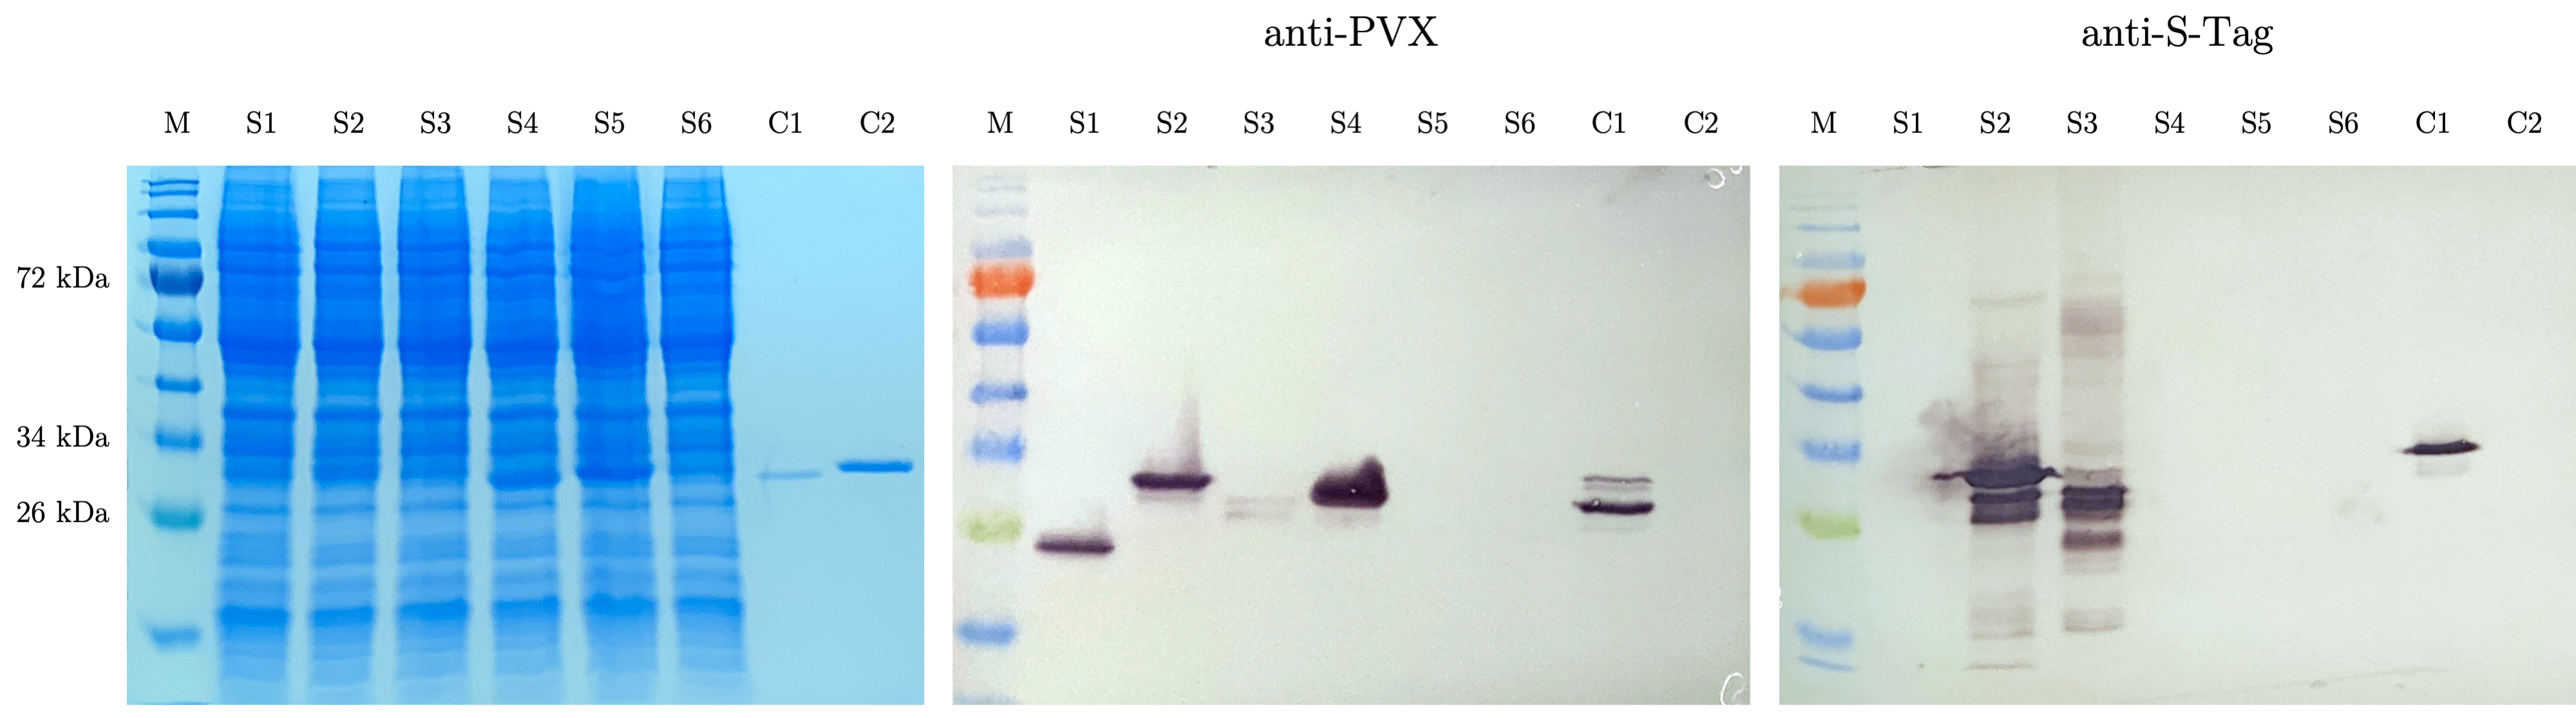
\includegraphics{lab/blot_alice.png}
\caption{\textbf{Coomassie Gel and Western Blot images following ALiCE expression.} Samples were taken from the cell-free reaction mix of the constructs d29-A (S1), S-Tag-A (S2), S-Tag-B (S3), PVX CP (S4), Strep-eYFP (S5), and the non-template (S6). The controls used were purified Strep-eYFP (C1), and S-Tag-PVX virions (C2). The marker was NEB Color Prestained Protein Standard, Broad Range (10-250 kDa). In the Western Blot, the anti-PVX antibody creates signals for samples from d29-A, S-Tag-A, PVX CP, the control S-Tag-PVX, and a faint signal for S-Tag-B. The anti-S-Tag antibody leads to signals for S-Tag-A, S-Tag-B, and S-Tag-PVX. }
\label{fig:blot_alice}
\end{figure}

\begin{figure}
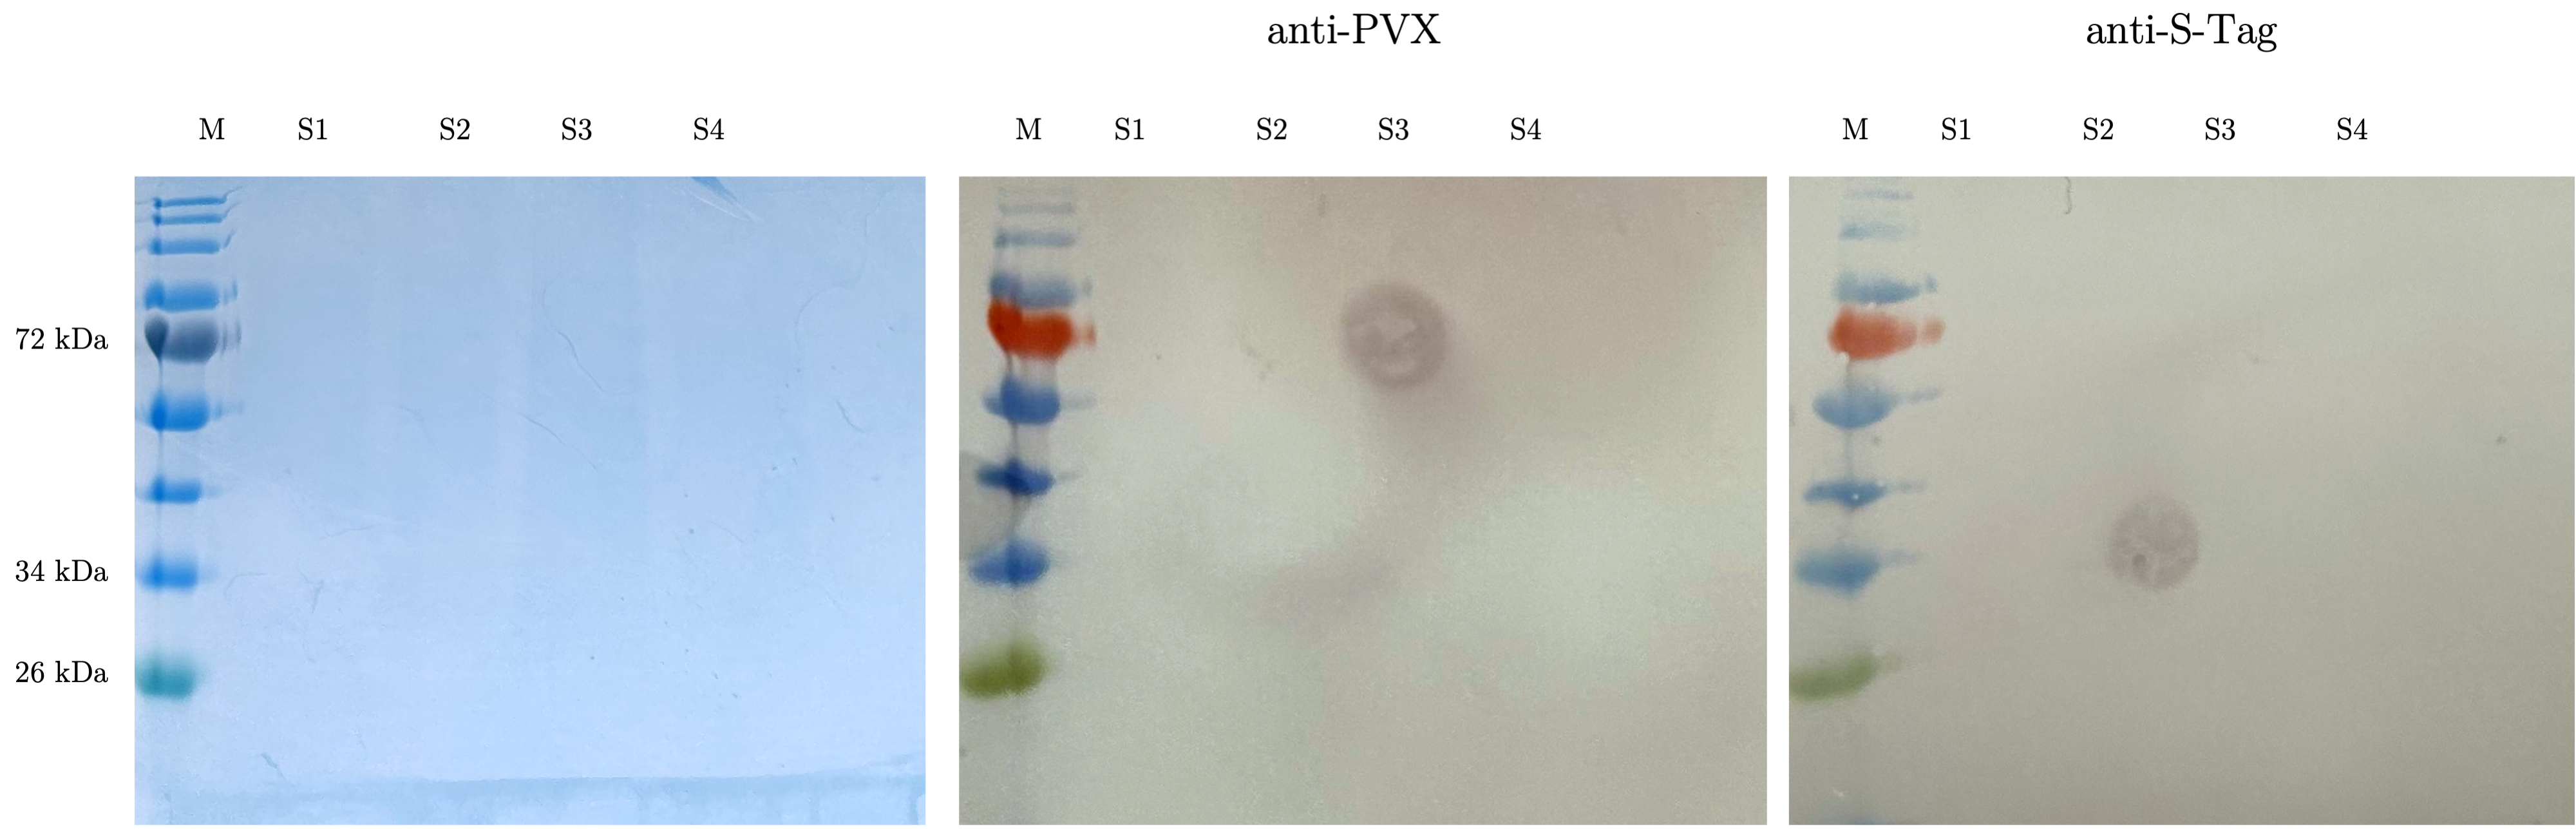
\includegraphics{lab/blot_capto_repetition.png}
\caption{\textbf{Coomassie Gel and Western Blot images following CaptoCore Purification.} Samples were taken from the concentrated CaptoCore flow-through for the constructs d29-A (S1), S-Tag-A (S2), S-Tag-B (S3), and PVX CP (S4). No control was used in the experiment. The marker was NEB Color Prestained Protein Standard, Broad Range (10-250 kDa). The blot created no signal for any of the samples. }
\label{fig:blot_capto_repetition}
\end{figure}


\label{subsection:elisa}
\subsubsection{ELISA}
For a quantitative analysis of the cell-free protein expression, an ELISA was performed on the samples, using both the anti-PVX antibody, and the anti-S-Tag antibody. 

The calibration measurements for the anti-PVX antibody show saturation at protein concentrations larger than \SI{100}{\nano\gram\per\milli\litre}. The four calibration samples below that threshold follow a linear trend 
\begin{equation}
\text{OD} = \SI{6.5}{\micro\litre\per\nano\gram} \cdot c
\end{equation}
with a coefficient of determination of $R^2=0.90$ (\autoref{fig:elisa_calib}). The measurements from the samples yielded significant OD values for d29-A, S-Tag-A, and PVX CP, and no significant signal for S-Tag-A and the non-template H\textsuperscript{2}O from the ALiCE expressions (\autoref{tab:sample_values_elisa_anti_pvx}). For d29-A, S-Tag-A, and PVX CP, the measured ODs of the different dilutions were almost identical, with an OD of ~0.2 for d29-A, 0.22 for S-Tag-A, and ~0.87 for PVX CP. Due to this, the back-calculated concentrations using the linear model and the dilution factors vary over the two dilutions. Calculations based on the stronger diluted samples yield to concentrations of \SI{30\pm 5}{\micro\gram\per\milli\litre} for d29-A, \SI{33\pm 4}{\micro\gram\per\milli\litre} for S-Tag-A, and \SI{134\pm 4}{\micro\gram\per\milli\litre} for PVX CP. 

For the anti-S-Tag antibody, calibration was sub-linear for low concentrations, but followed a linear trend for the whole sample range up to \SI{1500}{\nano\gram\per\milli\litre}. The linear model was calculated as 
\begin{equation}
\text{OD} = \SI{0.9}{\micro\litre\per\nano\gram} \cdot c
\end{equation}
and yielded a coefficient of determination of $R^2 = 0.98$ (\autoref{fig:elisa_calib}). As for the anti-PVX antibody, the sample OD measurements were highly similar for the 1:500 and 1:1000 dilutions (\autoref{tab:sample_values_elisa_anti_s_tag}), with significant ODs of 2.4/2.2 (1:500/1:1000)  for S-Tag-A and 1.5/1.1 (1:500/1:1000) for S-Tag-B. The samples of d29-A, PVX CP, and the non-template control showed no significant absorbtion. Following back-calculation of the stronger dilution, the concentration for S-Tag-A was evaluated as \SI{2400\pm 90}{\micro\gram\per\milli\litre}, and for S-Tag-B as \SI{1200\pm 100}{\micro\gram\per\milli\litre}.

\subsubsection{Electron Microscopy}
For clarification whether the constructs were able to form particles, the purified samples from the constructs d29-A, S-Tag-A, S-Tag-B, PVX CP, and a control of S-Tag-CP-PVX particles expressed in plants were analyzed using transmission electron microscopy. The construct S-Tag-A and the cell-free expressed PVX CP showed some clumped, darker areas, that are also present in the non-template control (\autoref{em_overview}). The TEM images for d29-A showed little to no larger structures. For the control of S-Tag-PVX virions, a network of flexible filamentous rod-shaped particles with diameters of about ~\SI{17}{\nano\meter} (varying length, ~\SI{600}{\nano\meter}) was visible. 

\begin{figure}
\includegraphics{lab/em_overview.png}
\caption{\textbf{TEM images of samples following CaptoCore purification. } Images are shown for the constructs d29-A (a), S-Tag-A (b), S-Tag-B (c), PVX CP (d), a control sample of S-Tag PVX virions (e), and a sample from ALiCE reaction mix using a non-template, captured using the anti-PVX antibody (f). The image for the non-template sample was provided by the Institute of Molecular Biotechnology. The black bars mark a length of \SI{500}{\nano\meter}. The control sample shows a network of flexible, filamentous particles. The sample from S-Tag-A showed two rod-like structures over all images. Other samples did not contain signs of tubular particles. }
\label{fig:em_overview}
\end{figure}

The images for S-Tag-B were similar in appearance to those of the non-template control, but included two rod-like structures, one of which appeared flexible with a diameter of ~\SI{15}{\nano\meter} (~\SI{760}{\nano\meter} length), and the other appearing more rigid with a diameter of ~\SI{24}{\nano\meter} (~\SI{850}{\nano\meter} length) (\autoref{fig:em_particles}). 

\begin{figure}
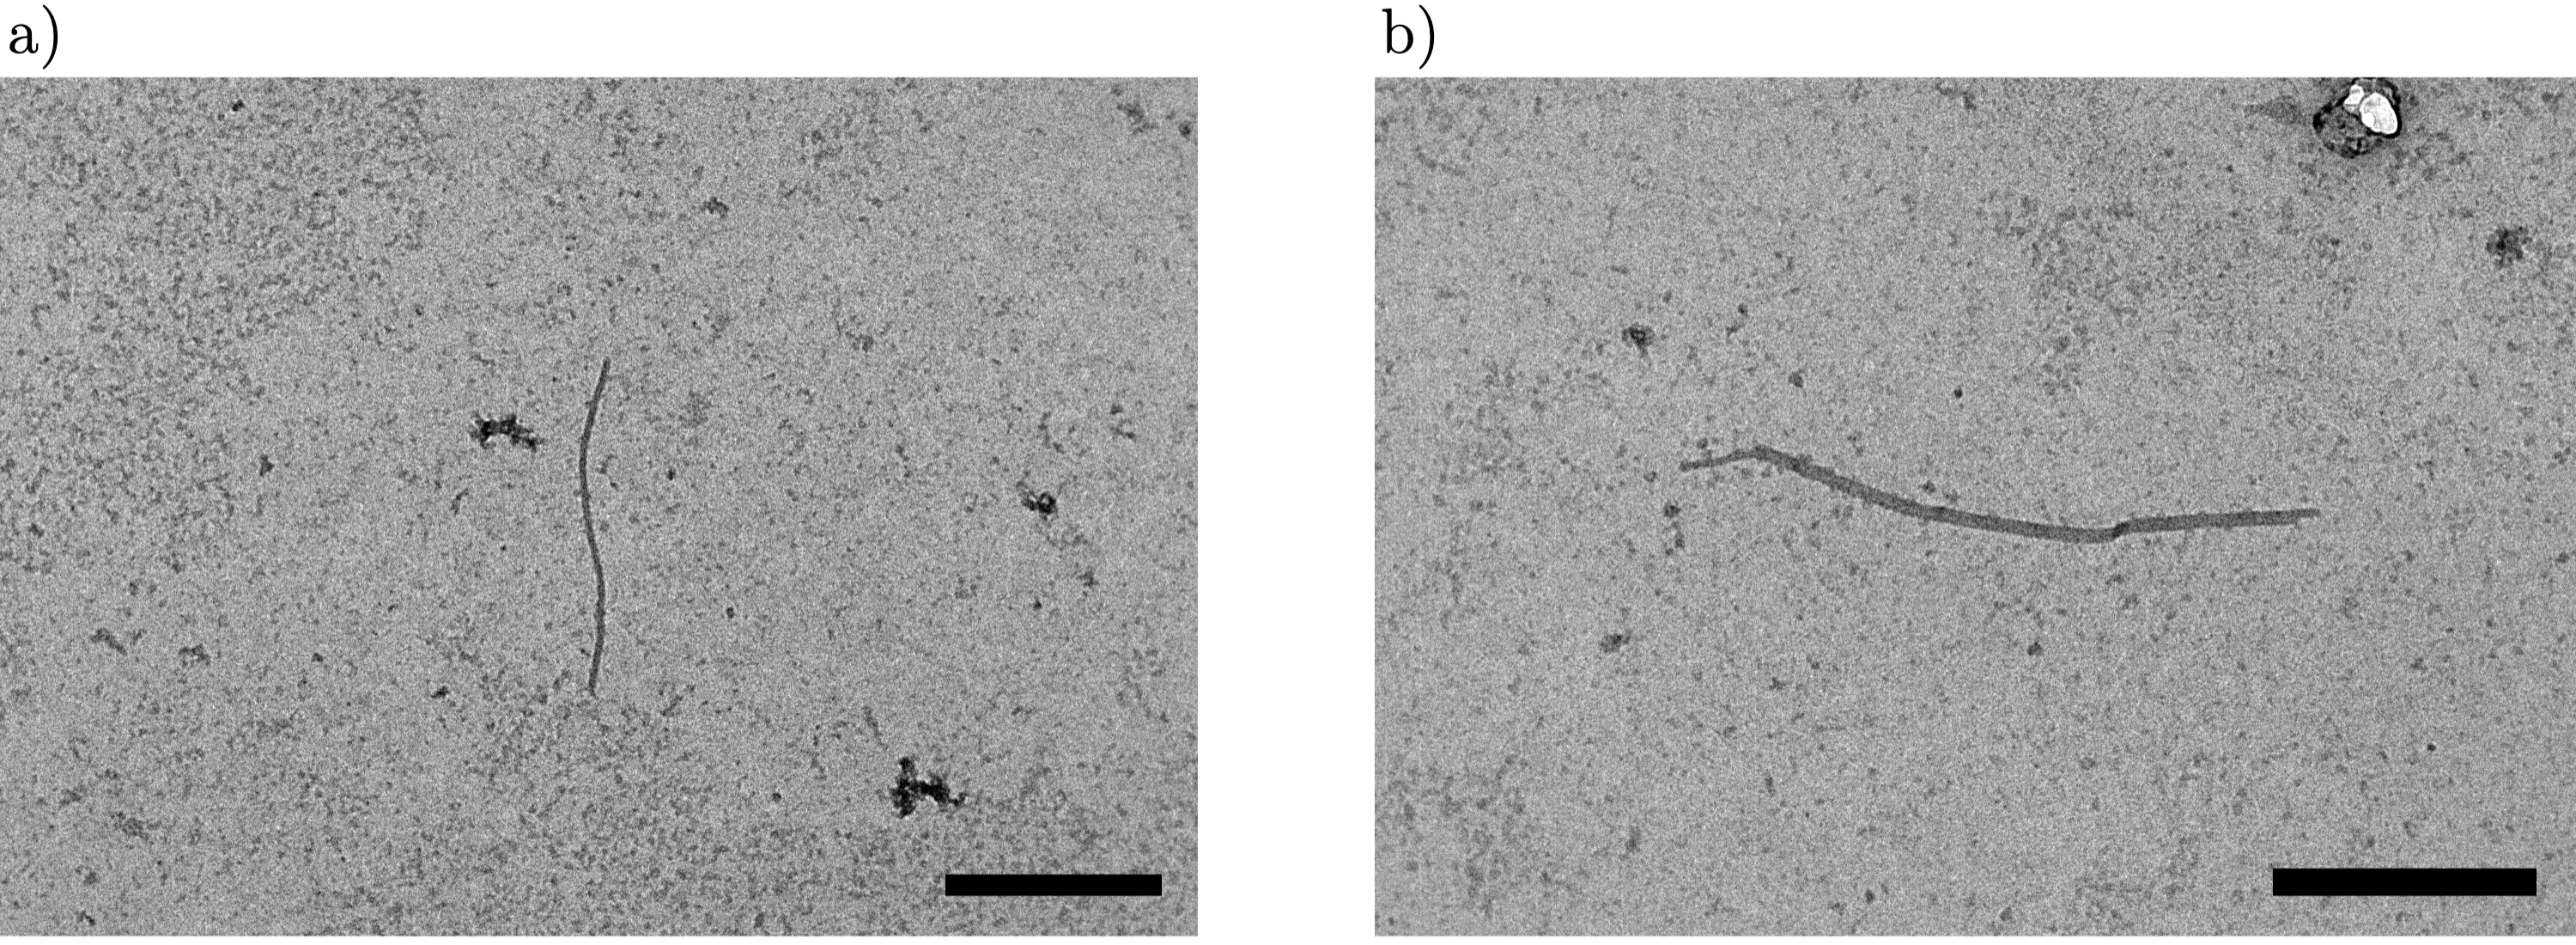
\includegraphics{lab/em_particles.png}
\caption{\textbf{TEM images of rod-like structures in the sample of the design S-Tag-B. } The two shown images display the only tubular structures found in the sample. The structure in (a) appears flexible with a diameter of ~\SI{15}{\nano\meter} and a length of ~\SI{760}{\nano\meter}, while the structure in (b) appears more rigid with a diameter of ~\SI{24}{\nano\meter} and a length of ~\SI{850}{\nano\meter}.}
\label{fig:em_particles}
\end{figure}

\subsection{DNA Cloning}
DNA cloning was concluded by sequencing of the plasmids and the calculation of the yield from the midi preparation. The full agreement of the sequencing result with the designed sequences enables further use of the plasmids in cell-free expression. The yields of the midi preparation are slightly lower than the manufacturer's reported typical yield of \SI{500}{\micro\gram}, but still high enough to allow for use in cell-free expression after concentration. 

\subsection{Protein Expression}
\subsubsection{eYFP Yield by Fluorescence}
Following cell-free expression, the protein yield of the batch was estimated by fluorescence measurements of the Strep-eYFP reaction setup. The determined concentration of \SI{0.3}{\milli\gram\per\milli\litre} is significantly lower than the manufacturer's reported typical yield of at least \SI{2}{\milli\gram\per\litre}. Typical reasons for low lysate performance, as stated by the manufacturer, are an inappropriate amount of plasmid DNA, poor oxygenation, or expired lysate. As for the plasmid DNA, the manufacturer explains that the optimal amount varies for each protein and should be determined by testing. Potentially, use of less DNA could improve the yield. Oxygenation in this setup was provided through a hole in the reaction tube's lid. An optimal oxygen supply could be established by using the dedicated perforated lids shipped with newer versions of the lysate. Use of newer lysate might also lead to a higher yield, since deterioration of the kit's components is a known issue 

\subsubsection{Coomassie Staining and Western Blot}
Evaluation of the cell-free expression's qualitative success, as well as of the CaptoCore chromatography, was conducted through Western Blots using an anti-PVX antibody and an anti-S-Tag antibody.

After the Coomassie staining of the ALiCE reaction mixture, the samples d29-A, S-Tag-A, and S-Tag-B, showed no notable difference from the non-template control, while the tracks containing expression mix from the PVX CP and the Strep-eYFP setup display bands at molecular weights matching the control. This could imply a lower yield in these setups. However, the bands from other proteins in the lysate provides bad contrast, and visual differences might simply be caused by the fact that the bands are at slightly different heights than those of Strep-eYFP, and possibly worse to distinguish from the background. Further, the control S-Tag-CP-PVX only displays a faint band as well, reinforcing that there is no sure implication on the yield. 

The anti-PVX Western Blot shows defined bands for d29-A, S-Tag-A, and PVX CP, but only a very faint band for S-Tag-B. This could be due to a lower yield for S-Tag-B, or less avidity of the anti-PVX antibody against the protein, given that in only has \SI{0.53}{\percent} sequence identity to the wild type. For all samples and the control S-Tag-CP-PVX, the migration of distance suggested a molecular weight higher than the theoretical one. For PVX particles from plants, this is a well-known phenomenon and partly due to specific glycosylations of the proteins \cite{pvx_glycosylation}. However, glycosylation of the ALiCE samples is unlikely, since they were expressed through the cytosolic pathway. The discrepancy with the theoretical weights might imply partial aggregation. Binding of the anti-PVX antibody against the d29-A and S-Tag-A and the faint signal for S-Tag-B could indicate that the coat proteins partially folded into the desired shape. Having said that, the anti-PVX antibody is polyclonal and it is not clear whether its epitopes are specific to the proteins fold. 

In the Western Blot using the anti-S-Tag antibody, both samples S-Tag-A and S-Tag-B show a strong signal, implying that the antibody has high avidity against them. The signal is not constrained to the migration distance as seen in the anti-PVX blot, but is faintly visible through most of the track. Signal at larger molecular weights might stem from aggregates, while signal at lower molecular weights suggests the existence of smaller protein parts containing an S-Tag, possibly through partial degradation of the protein while boiling the samples. 

Following CaptoCore purification, no discernible bands were visible in the Coomassie gel or the Western Blot. The signals in the first iteration of the Western Blot likely arose from column resin permeating the filter and carrying protein with it. However, it is also possible that the signal in the first batch actually stemmed from specific or unspecific protein complexes that did not form in the second batch. This is rendered unlikely since, in the first blot, the wild type PVX CP also showed a signal, even though it is known to not assemble in absence of its genome \cite{juli_sagt_keine_assembly}. In any case, the Western Blot following CaptoCore purification indicates that there were little to no assembled complexes in the reaction mixture. 

\subsubsection{ELISA}
For a quantitative analysis of the cell-free expression of d29-A, S-Tag-A, S-Tag-B, and PVX CP, ELISAs using both anti-PVX and anti-S-Tag antibodies were conducted. 

In both cases, the optical densities of the samples were almost identical for the 1:500 and the 1:1000 dilution. This might be caused by other proteins in the lysate saturating the binding capacity of the microwell plate, even at the stronger dilution, and thus rendering only the proportion of the specific protein in the reaction mixture relevant. Under this assumption, the result from the 1:1000 dilution would be more significant, even though in general stronger dilutions should be tested to get a better estimate. 

Using the 1:1000 dilution, the highest protein concentration in the anti-PVX ELISA was observed for the PVX CP, with a calculated concentration of \SI{134}{\micro\gram\per\milli\litre}. This is less than half the value measured for Strep-eYFP expression by the lysate. A possible cause is lower expression or quicker degradation of the protein in the reaction mixture. A different reason could be that the antibody has higher avidity for the assembled viral particles than for the PVX CP in the ALiCE expression mix, which are known to not assemble without specific RNA present \cite{pvx_assembly}. This is plausible, since the antibody was generated by rabbit immunization against viral particles. For the constructs d29-A, S-Tag-A, and S-Tag-B, the anti-PVX ELISA leads to lower calculated concentrations of about \SI{30}{\micro\gram\per\milli\litre} for d29-A and S-Tag-A, and no discernible signal for S-Tag-B. This could also be due to lower avidity of the antibody towards the adapted sequences. The missing signal for S-Tag-B is consistent with the anti-PVX Western Blot, which showed only a very faint line for S-Tag-B. 

Using the anti-S-Tag antibody, only the samples from S-Tag-A and S-Tag-B had significant optical densities. The back-calculated concentrations of \SI{2.4}{\milli\gram\per\milli\litre} and \SI{1.2}{\milli\gram\per\milli\litre} are very high, and unlikely given the measured expression of only \SI{0.3}{\milli\gram\per\milli\litre} for the Strep-eYFP ALiCE control setup. Possibly, the anti-S-Tag antibody has considerably higher avidity against protein monomers than for the assembled particles in the calibration samples. This could explain the high optical density, since the faint signal in the CaptoCore after the Western Blot implies that little to no protein in the ALiCE setup assembled. Notably, the anti-S-Tag antibody is not explicitly labeled as being suitable for ELISA, so the high signal might also be due to this, even though the calibration showed a linear trend with high determination.

\subsubsection{Electron Microscopy}
The electron microscopy, conducted to analyze whether assembled particles were present in the purified ALiCE reaction mixture, showed no signs of VLP formation for the constructs d29-A, S-Tag-A, as well as the expressed PVX CP. The visible dark clumps in the images also appear in the non-template control and are thus likely not related to the specific expressed protein, but rather to other components of the lysate that passed the CaptoCore column. This observation is in line with the absence of a signal in the Western Blots after the purification. 

The control sample of S-Tag-PVX virions clearly showed the filamentous, flexible structure of PVX virions as described by Grinzato et al. The measured size of \SI{17}{\nano\meter} in diameter and about ~\SI{600}{\nano\meter} in length agree with values from literature of a diameter of \SI{15}{\nano\meter} and a modal length of ~\SI{500}{\nano\meter}. 

One of the two rod-like structures found in the purified reaction mix of S-Tag-B also has the shape of PVX virions, with a measured diameter of \SI{15}{\nano\meter}, a length of \SI{760}{\nano\meter}, and a flexible structure. The other structure is thicker than PVX, with a measured diameter of \SI{24}{\nano\meter}. Both could potentially indicate assembly of S-Tag-B coat proteins into helical complexes. However, the fact that only two of those structures were found in the sample make this result unsure. Clarification on whether or not these structures are actually made up of S-Tag-B monomers could be achieved by using immunoelectron microscopy (exemplary image in \ref{fig:em_immuno_labeling}).

% Successful expression
% designs with PMPNN and filtered through AlphaFold performed well in silico evaluation using GROMACS
% designs d29Orange and S-Tag Orange showed response to anti-PVX, indicating 
%   correct fold
% no real particles to see, S-Tag-B would need to be validated by immunoelectron microscopy
% missing assembly not too surprising: 608 designs for experimental characterization and found using size-exclusion chromatography (SEC) that at least 87 had oligomerization states closely consistent with the design models  (RFdiffusion)
% AI has opened the doors for Protein design, but with current models, much testing necessary
% this could be helpful here, but without RFdiffusion, low diversity in sample generation
% if fixed (possibly through fixing the improper distribution), could enable larger scale design evaluation
% ALiCE lysate helpful for creating large number of designs
% an intermediate number, like a few hundred designs, could be reasonably assessed with current methods
% Might be helpful to try out Baker protocols from RFdiffusion, which can be conducted in 96 well plates
% All in all: Work proposed new methods for design and evaluation for a new task of symmetry fulfillment. Designs showed in silico success, but experimental evaluation wasn't affirmative
% If diversity of designs can be increased, higher-throughput methods could shed light on this.

This work introduced novel computational methods to design and evaluate proteins tailored to a specific geometric architecture. The design and filtering process, using modified implementations of ProteinMPNN and AlphaFold 3, showed promising results at in silico evaluations using GROMACS. Protein expression of the constructs could be confirmed. Notably, binding of anti-PVX against the designed coat proteins, even with a faint signal for the construct S-Tag-B that shares only \SI{53}{\percent} sequence identity to the wildtype, could imply partially correct folding of the sequence to the desired monomer structure. 

Despite this, assembly of the particles could not be confirmed through size exclusion chromatography and transmission electron microscopy. Nonetheless, failure to observe particle assembly does not necessarily preclude the utility of the methods employed. In similar assays for design of symmetric homooligomers carried out by Watson et al., only 87 out of 608 designs showed the desired oligomerization state \cite{RFdiffusion}. While modern AI models for protein design allowed for design campaigns that were previously impossible, currently available models have success rates that still require a larger number of designs to fulfill the desired fold. 

The primary limitation for scaling up the current design methods is that RFdiffusion failed to generate novel backbone structures for the geometry. Sole use of ProteinMPNN strongly limits the diversity of the designs, making a success by simple upscaling unlikely. The success of RFdiffusion in symmetric design for point group symmetries makes it plausible that use for other symmetries is possible. Failure by the method used here could be due to the strong effect of translation on the distribution in early stages of the diffusion process. This could be mitigated by gradually increasing the translational symmetry over the course of the denoising process, similar to how the symmetry enforcement effects diffusion in AlphaFold 3.

If a higher diversity of designs can be achieved, an increase in the number of experimental evaluations could be able to find a suitable protein. The experimental methods used in this paper could realistically be used for a higher number of 50 to 100 designs. The cell-free expression system in particular allows for simple and fast protein expression. Another noteworthy option are the protocols that were successfully employed for the evaluation of symmetric homooligomeric designs by RFdiffusion \cite{RFdiffusion}. These allow for plasmid assembly, transformation, expression, and purification in microplates, as well as employment of automated size exclusion chromatography of evaluation of the oligomeric state. Using these protocols, experimental evaluation could be carried out with a considerably higher throughput. 

All in all, while the computational methods proposed in this work did not lead to the desired assembly into particles, the partial success of the designs demonstrates their potential. With modifications to the design process and an increased focus on high-throughput evaluation, AI-driven methods may yet enable the construction of functional PVX VLPs.